\documentclass[tikz, border=5pt]{standalone}
\usetikzlibrary{arrows.meta, shapes, positioning, decorations.pathmorphing}

\tikzset{
  spring/.style = {
    decoration = {aspect=0.3, segment length=3mm, amplitude=3mm, coil},
    decorate
  }
}

\begin{document}
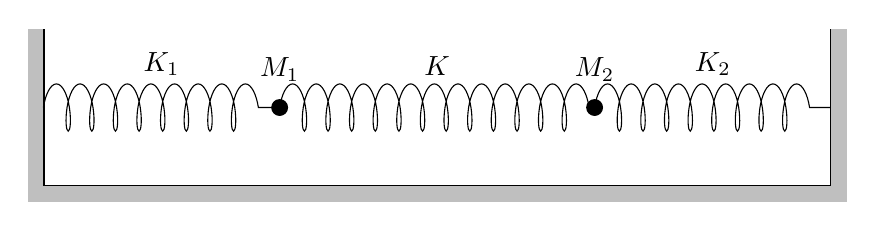
\begin{tikzpicture}

    %% Hamiltonian formulation

    % Walls
    \draw[thick] (-5,0) -- (5,0);
    \draw[thick] (-5,0) -- (-5,2);
    \draw[thick] (5,0) -- (5,2);
    \fill[gray!50] (-5,0) rectangle (-5.2,2);
    \fill[gray!50] (5,0) rectangle (5.2,2);
    \fill[gray!50] (-5.2,-0.2) rectangle (5.2,0);

    % Masses
    \draw[fill=black] (-2,1) circle (0.1) node[above, yshift=6] {\(M_1\)};
    \draw[fill=black] (2,1) circle (0.1) node[above, yshift=6] {\(M_2\)};

    % Springs
    \draw[spring] (-5,1) -- (-2,1) node[midway, above, yshift=8] {\(K_1\)};
    \draw[spring] (-2,1) -- (2,1) node[midway, above, yshift=8] {\(K\)};
    \draw[spring] (2,1) -- (5,1) node[midway, above, yshift=8] {\(K_2\)};

\end{tikzpicture}
\end{document}
